%!TEX root = ../Thesis.tex

\def\chapdir{./ChapterLiteratureReview}

\chapter{Literature Review} \label{ch:litreview}



\section{Position Requirements}
- how/why to use position for applications\\
- absolute vs relative\\
- why use relative positioning\\
- knowing where you are positioned is important for data gathering, motion detecting and tracking, path planning\\
- formation flying, drones\\
\section{Relative Positioning Technology}
- line of sight methods\\
- pre-setup requirements\\
- long calibration setup?\\


- last one being GNSS
\section{GNSS Operational Components}
\subsection{Space Segment}
- current GNSS: explain GPS, GLONASS, galelao, chinese one constellations and how it works
- what orbits are they in and why?: altitude\\
inbetween the two radiation belts?
\subsection{User Segment}
- typical accuracy for civilian accessable gps\\
- military has more precise stuff\\
- lower cost receivers have only one frequency band, error in timing\\
Unfortunately, low cost GNSS receivers rarely provide official access to the GNSS raw data. Previous studies have used customised bluetooth headsets or customised android platform mobile phones to investigate algorithms on low-cost GNSS receivers. More expensive receivers do allow raw data to be utilised, however they also provide other mechanisms such as duel frequencies and more accurate clocks, rendering the new algorithm *obtuse*. The mindset of *crowd-sourcing*/customising/flexible technology is changing the way manufactures build GNSS receivers. The new Android OS platform Nougat 7.0 provides the developer raw GNSS data at the software level.  

\subsection{Control Segment}


\section{GNSS Satellite Signals}
There are two sets of signals that are sent from every satellite, the pseudorandom binary sequence (PRN code) and the navigation message. 

The PRN code is intentionally complex to know which cycle is being received

L1 frequency of 1575.42 Mhz  - code phase
Course Acquisition (C/A) code is transmitted on the L1 frequency as 1.023 MHz signal using a bi-phase shift keying modulation technique.
Navigation message sent at 50 bits per second  

However the receiver does not know which cycle in the PRN code it is looking at. To resolve this ambiguity (how many 1 ms) requires decoding of the data message and analysing the pattern of bits.
\url{https://ocw.mit.edu/courses/earth-atmospheric-and-planetary-sciences/12-540-principles-of-the-global-positioning-system-spring-2012/lecture-notes/MIT12_540S12_lec7.pdf}

- civilian GNSS using duel frequency, send CDMA, how decryption works\\
- what is psudorange?\\
- what is carrier phase\\
- clock bias\\


%The first row shows a C/A code with 1,023 chips; the total length is 1 ms. The second row shows a navigation data bit that has a data rate of 50 Hz; thus, a data bit is 20 ms long and contains 20 C/A codes. Thirty data bits make a word that is 600 ms long as shown in the third row. Ten words make a subframe that is 6 seconds long as shown in row four. The fifth row shows a page that is 30 seconds long and contains 5 subframes. Twenty-five pages make a complete data set that is 12.5 minutes long as shown in the sixth row. The 25 pages of data can be referred to as a superframe http://read.pudn.com/downloads85/ebook/326017/Fundamentals%20of%20Global%20Positioning%20System%20Receivers/booktext05.pdf (pg77)

% resources about the signals:
% http://geoconnect.com.au/gps-signals-l1-l2-l5/
% http://www.trimble.com/gps_tutorial/dgps-advanced4.aspx
% https://www.e-education.psu.edu/natureofgeoinfo/c5_p14.html
% http://what-when-how.com/gps/gps-details/
% https://www.e-education.psu.edu/geog862/node/1742
% https://ocw.mit.edu/courses/earth-atmospheric-and-planetary-sciences/12-540-principles-of-the-global-positioning-system-spring-2012/lecture-notes/MIT12_540S12_lec7.pdf
% http://read.pudn.com/downloads85/ebook/326017/Fundamentals%20of%20Global%20Positioning%20System%20Receivers/booktext05.pdf
% http://www.navipedia.net/index.php/GPS_Navigation_Message

\section{The GNSS concept}
The base concept behind identifying the position of something using GNSS is remarkably simple. Satellite W sends out a radio signal at time X and it's position Y which the user received at time Z. The time difference is used to calculate the distance from the satellite's position. With this information from multiple satellites, the position of the user is triangulated. 


- timing comparison between satellite and receiver to find psudeorange
- ECEF frame of reference
\subsection{2D case}
\subsection{3D case}
- NLLS solve spheres
- need 4 satellites minimum
- 


\section{GNSS Error Sources}
- how large
\subsection{Clock Errors}
- timing of received signal because of low cost clock on receiver. 
\subsection{Receiver Noise}
- antenna phase
\subsection{Ephemeris Errors}
- satellite position is approximated\\
- due to gravity effects of other gravitational sources/ non-spherical earth/ what model is used?\\
- how long is the ephemeris data accurate for?\\
- actual location of satellite, where it thinks it is is based on a prediction model so its not 100\% correct. what uncertainty in this location therefore vector is there?

\subsection{Atmospheric Effects}
- ionosphere and troposphere refraction - speed of propagation changes which alters the time of flight\\
\url{http://www.trimble.com/gps_tutorial/howgps-error.aspx} \\
The distance from a satellite to a user is calculated by the time difference when the radio signal was sent and when it was received. However, the speed of light is reduced when in the atmosphere compared to that in space.\\
The ionosphere is the upper layer of the atmosphere ranging from 50 to 500 km


\subsection{Mutlipath Interference}


\subsection{Sagnac Effect}


\subsection{Electrical Interference}
- space weather\\
- jamming?

\subsection{GNSS Error Summary}


\section{Multiple Receivers}
- problems arising with multiple receivers
- 

\section{Current GNSS algorithms}
- just reference implementation papers?
- algorithms to make it more accurate\\
- use for motion tracking\\
- performance vs cost trade off\\
(http://ieeexplore.ieee.org.ezproxy1.library.usyd.edu.au/document/7530542/)
\subsection{Standard Positioning Service}
- single frequency and multi frequency to remove atmospheric affects
\subsection{Differential GPS}
- explain what it is\\
- what setup is required \\
- abs vs rel \\
- degree of accuracy
\subsection{WAAS DGPS}

\subsection{SBAS  ?}

\subsection{Real Time Kinematic}

\subsection{Post Processing Algorithm}

\subsection{Single Frequency Precise Point Positioning (SF-PPP)}
Rademakers \textcolor{red}{how to say reference?} at University of Delft in the Netherlands developed a solution for finding the absolute position in open areas to a horizontal accuracy of 0.5 m. It uses a single frequency, single antenna low cost GPS receiver by connecting to the internet and using real time information to model all errors. The errors they corrected with the potential improvements are outlined in Table \ref{Table:SFPPP error table}. 
\begin{table}
\centering
\caption{Error Components and Potential Improvements for SF-PPP}
\label{Table:SFPPP error table}
\begin{tabular}{|l|l|}
\hline
\textbf{Error component} &\textbf{ Potential Improvement} \\\hline
 Ionosphere: Klobuchar model & 7 m \\\hline
 Troposphere: Saastamoinen model & 2.5 m \\\hline
Ephemeris data &  1 m \\\hline
 Satellite clock drift & 1.5 m \\\hline
 Differential code bias & 50 cm \\\hline
 Phase windup: rotation of the antenna & dm \\\hline
 Sagnac effect & 30 m \\\hline
 ROA: satellite orbit correction & up to 10 cm \\\hline
 Relativistic clock correction & up to 21 m \\\hline
 Moon-Earth interaction & 5cm (Hor) and 30 cm (Ver)\\\hline
\end{tabular}
\end{table}


\subsection{Duel-Epoch, Double-Differencing Model} \label{DEDD}
In the paper by the Institute of Software Integrated Systems, Vanderbilt University called \textit{High-Accuracy Differential Tracking of Low-Cost GPS Receivers}, Hedgecock and party developed a new algorithm for relative motion tracking for multiple receivers. They used low cost GPS receivers with access to raw measurement data to produce centimeter-scale tracking accuracy. Each receiver was shared the whole networks data and ran the localisation algorithm independently to avoid having a single point of failure.\\

The algorithm uses the change in carrier phase through time of each receiver to estimate the change in relative ranges between a satellite and two receivers. It does not require a reference satellite, a reference node or an integer ambiguity solution. It does require the clock bias for each receiver at each point in time as solved for by non-linear least squares for the absolute position before running the algorithm itself. To reiterate, it does not directly solve for the relative position but the relative motion. However, neither of the initial positions of the receivers need to be precisely known in order for he relative motion to be accurate. Due to the time dependency, consistent satellite locks of at least four satellites are required, otherwise reinitialisation must occur. The calculated change was projected onto the unit direction vector from receiver to satellite. The system of these tracking equations was solved via least squares optimisation. \\

It uses the assumption that all satellites in the constellation are such a great distance from the surface of the Earth that the unit vector from both receivers are parallel to each individual satellite, as long as it is in the same geographical region. How far apart the receivers can be for this assumption to hold was not stated.\\ 




- how many receivers?\\
- why and how it aligns epoch\\
- uses difference in time for a single receiver to find change in motion.



- have this one last as it is the most similar\\
- needs instantaneous relative distance for first point, to speed up processing and make the first few time steps more accurate, also when locking onto new satellites


\subsection{Summary of Algorithms ?}

% types of algorithms making gps more accurate: table with columns = types of analysis, rows= types of algorithms
- dynamic tracking (need temporal measurements) vs static measurement - no temporal\\
- post processing vs pre-processing vs realtime\\
- ground structure vs free standing\\
- absolute vs relative\\
- accuracy (how much)\\
- computation time/space required\\
- what error is each method removing\\
- what piece of data it needs (if raw)\\
- calibration required\\
- robustness -> if a satellite goes out of view does it need to re-calibrate? passing information between receivers-> is one a reference? single point of failure



\section{Proposed Planar Intersection Algorithm}
Following the literature, the two main options for increasing the accuracy is extensive modelling of the errors, or some type of differencing algorithm. Error modelling requires external hardware, internet connection and extra computation time which increases the budget requirements. Whereas 



This new algorithm is derived from taking the difference in pseudorange between multiple receivers from one satellite and expressing the distances as planes.
\begin{figure}[h]
\centering
\caption{2D representation}
\label{fig:overall_singleS_multiR}
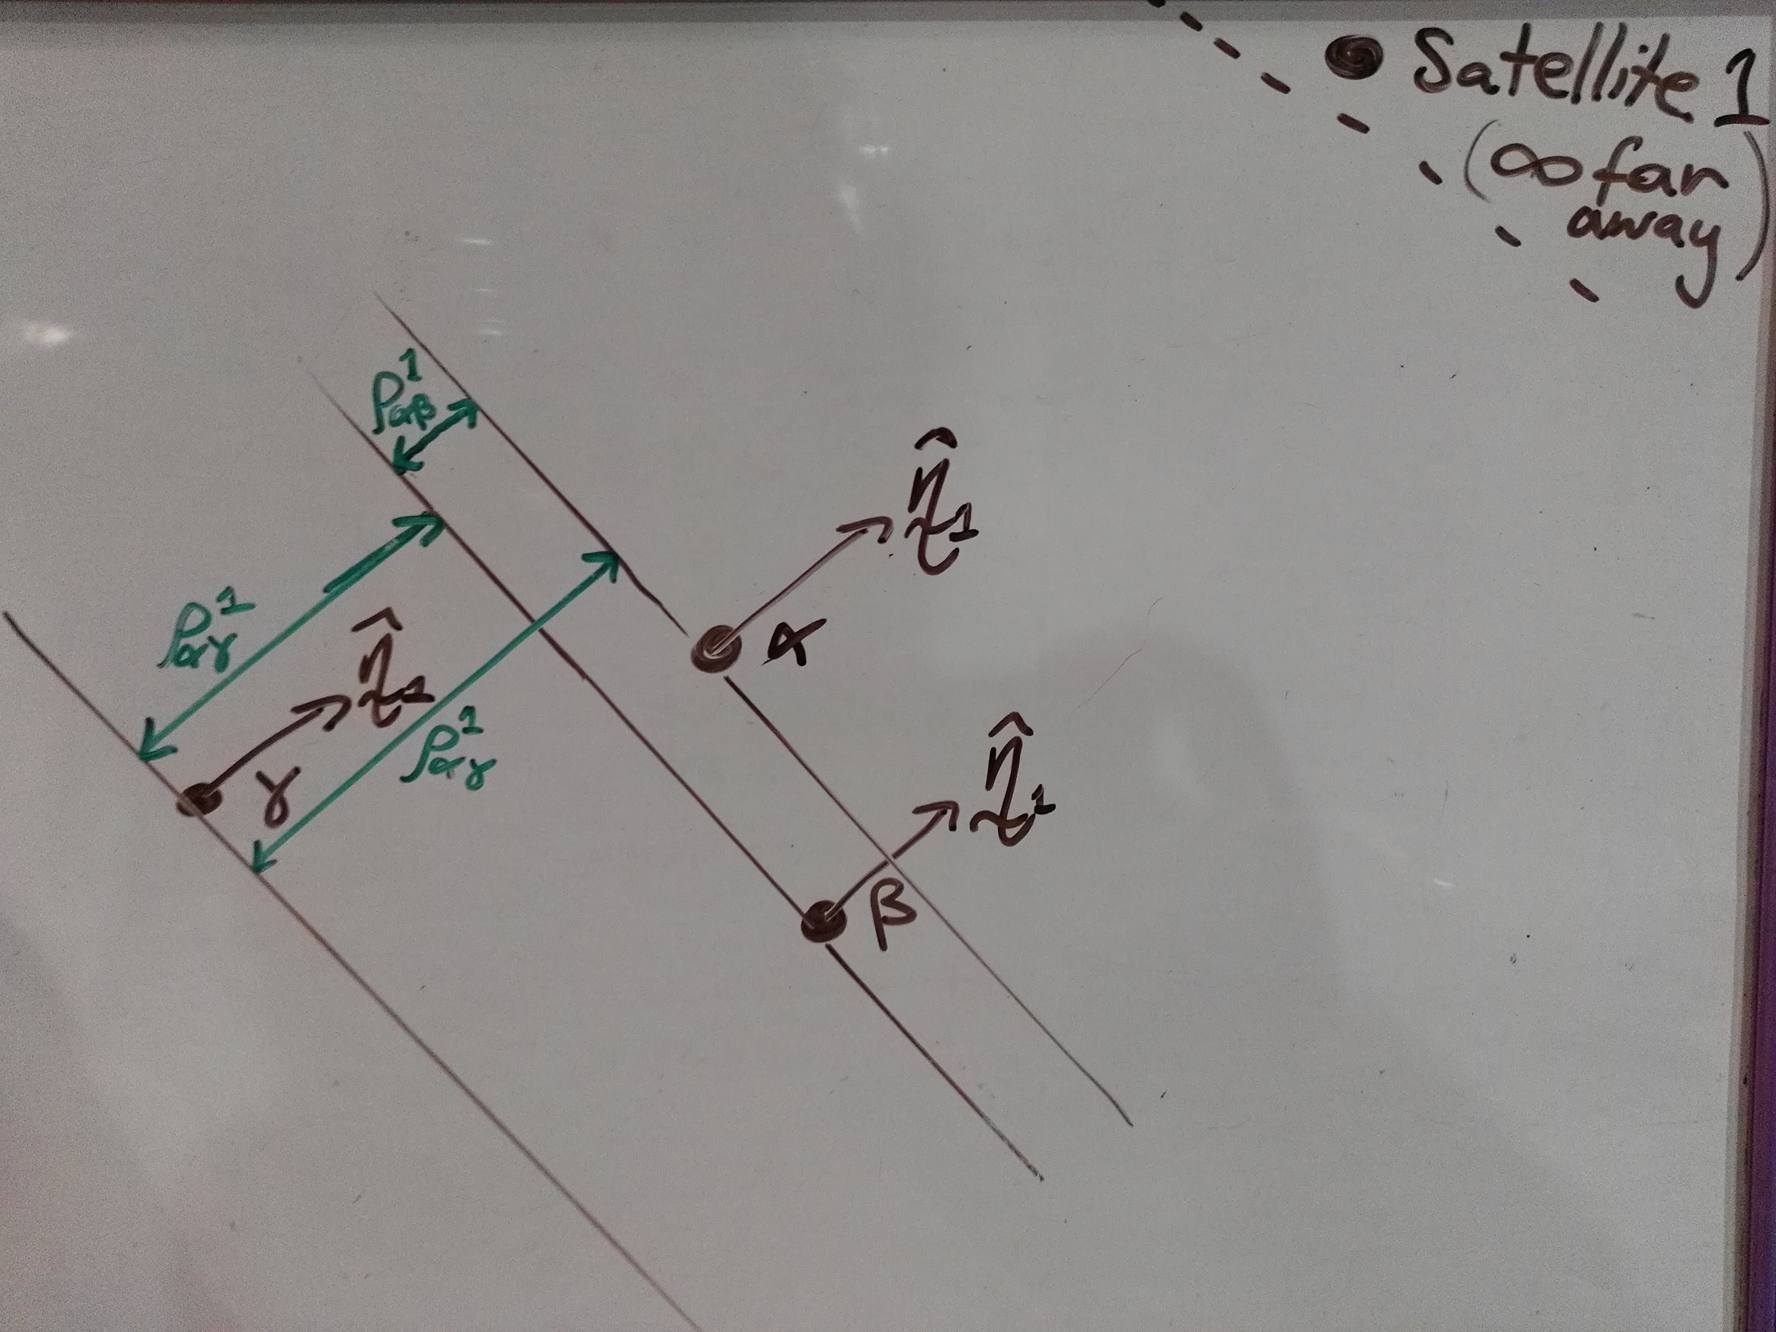
\includegraphics[width=0.7\linewidth]{ChapterLiteratureReview/overall_singleS_multiR.jpg}
\end{figure}

With multiple satellites in view, the intersection of planes for a particular receiver is the position of the receiver.
\begin{figure}[h]
\centering
\caption{}
\label{fig:overall_multiS_duelR}
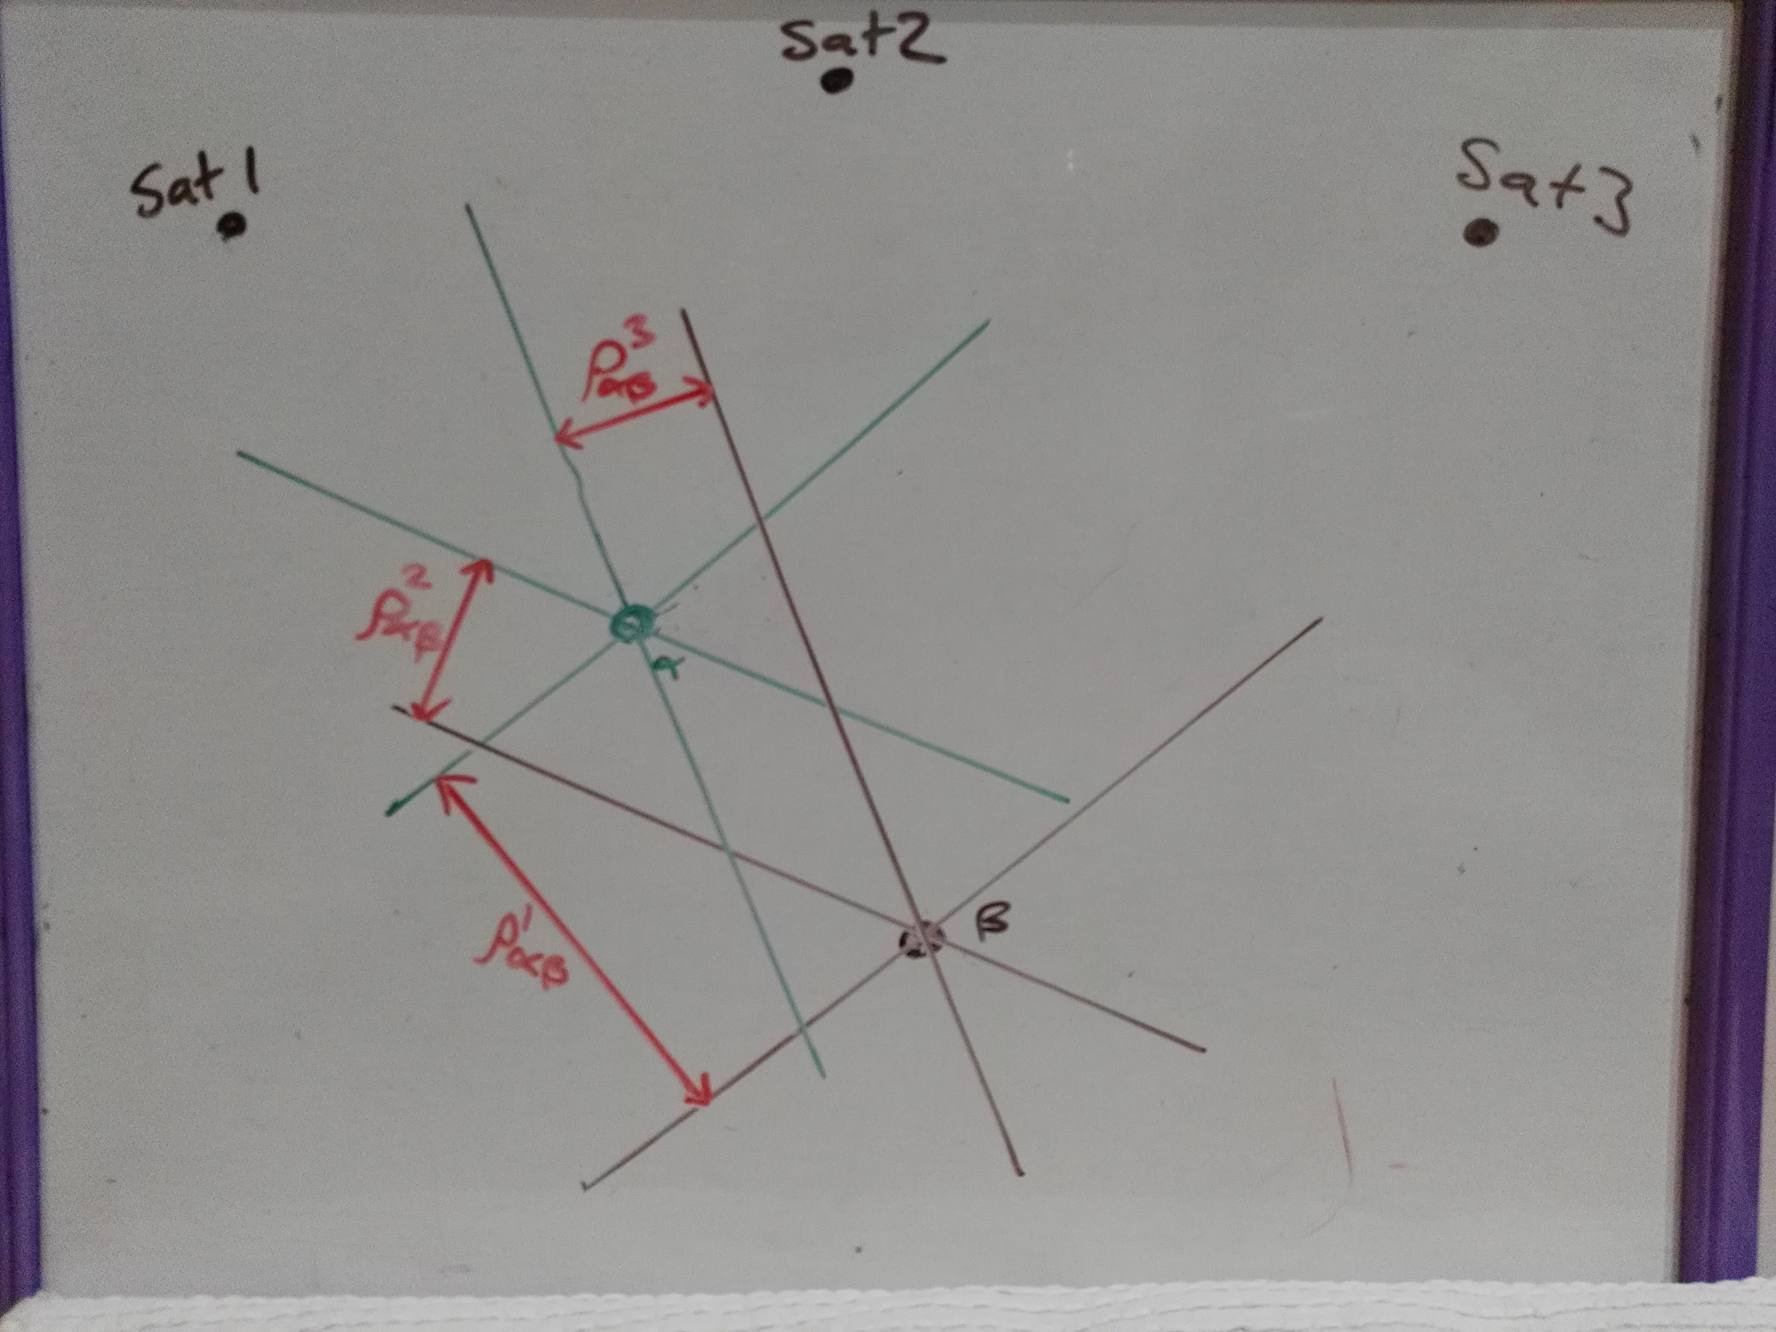
\includegraphics[width=0.7\linewidth]{ChapterLiteratureReview/overall_multiS_duelR.jpg}
\end{figure}

With this strategy, some of the errors that plague the absolute position are negated for the relative position. 
\begin{eqnarray}
\rho_i = \rho_n -cb_\omega + c(T_s + I_s+\nu_s+b_s)
\end{eqnarray}
where $\rho_n$ is the real range with the following sources of error; $b_\omega$ is the receiver clock bias, $T_s$ is the tropospheric error, $I_s$ is the ionospheric error, $\nu_s$ is the relativistic error and $b_s$ is the satellite clock bias.








% small






%??Topical organisation with inverted pyramid substructure
% \subsection{GNSS Localisation}
% Global Navigation Satellite System (GNSS) 
% - lower update rates $\approx$1Hz\\
% - accuracy/precision? not good enough for these applications\\
% - not good for indoor environments as signals are weak\\
% - used differentiated gnss to solve for integer ambiguity across multiple mobile platforms on the go \cite{GNSS_difftrack} \cite{GNSS_intamb}\\
% - multipath/atmospheric error estimation \\
% - multiple receivers across the multiplayers \cite{GNSS_multi} \\

% 	%% types of precision gnss locations 
% - double differentiating - requires same satellites
% - pvt position velocity and precise time